\documentclass{article}

\usepackage{graphicx}
\usepackage{tikz}
\usepackage{tikzsymbols}
\usetikzlibrary{calc,patterns,shapes.geometric}
\pagestyle{empty}
\usepackage[margin=0pt]{geometry}
\geometry{papersize={14in,12in}}

\def\centerarc[#1](#2)(#3:#4:#5){\draw[#1] ($(#2)+({#5*cos(#3)},{#5*sin(#3)})$) arc (#3:#4:#5);}

\begin{document}
	\begin{figure}
		\centering
		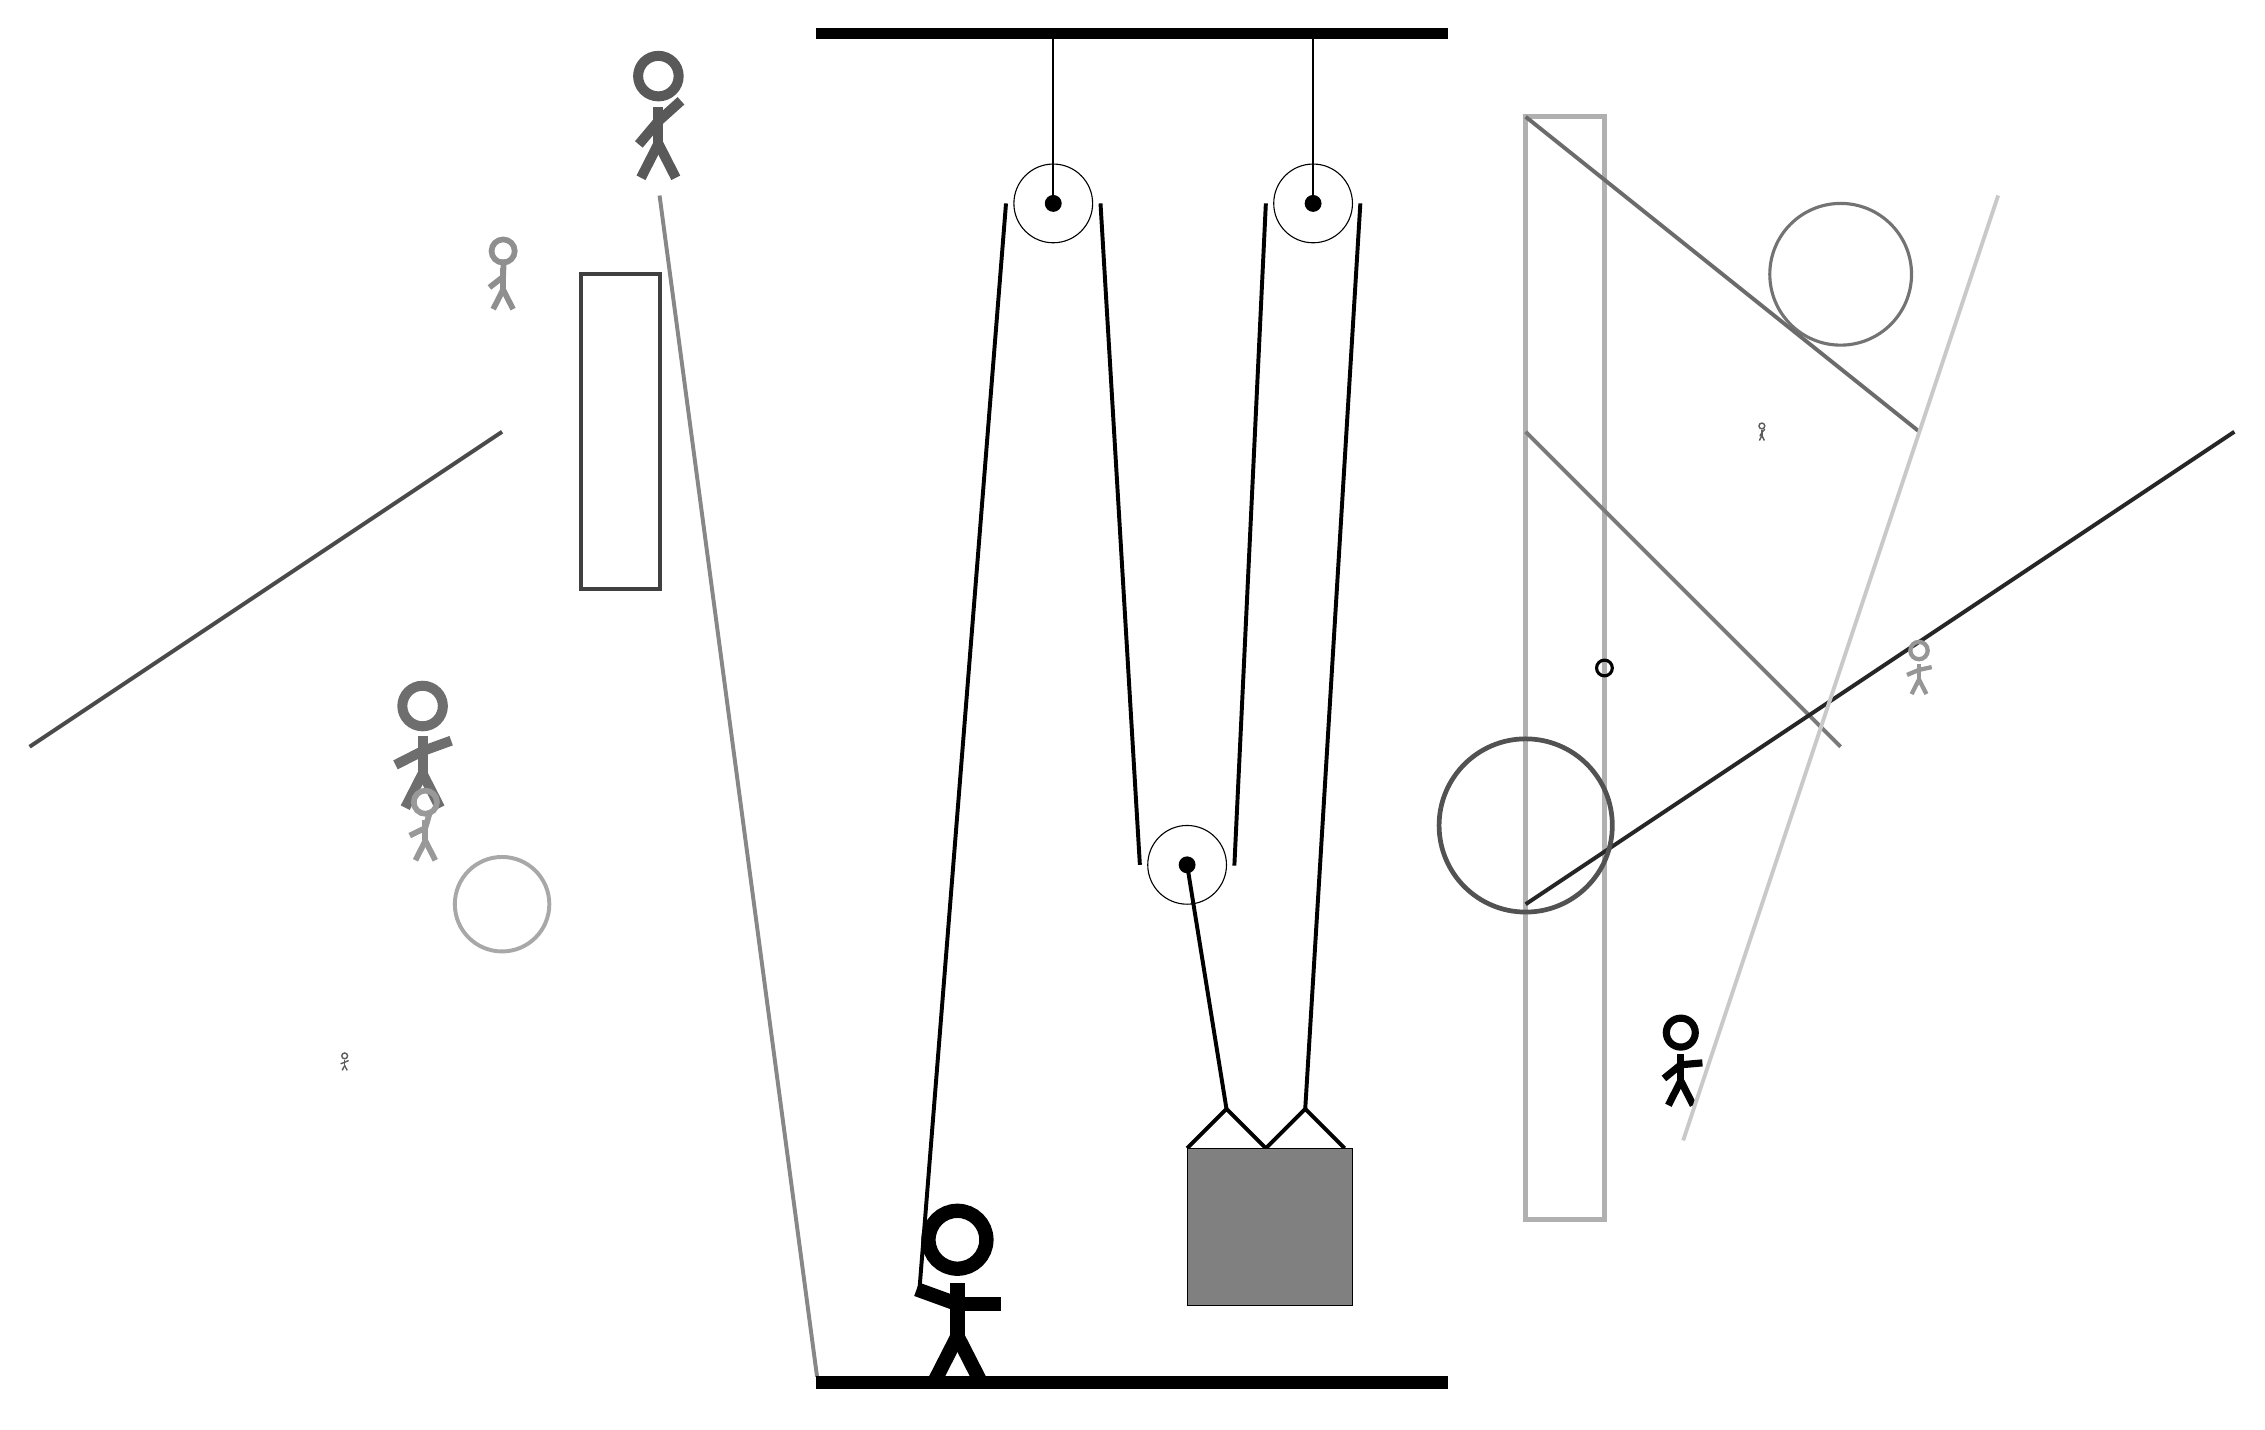
\begin{tikzpicture}
			%%%%% START %%%%%
			
			\draw[fill=black] (-2, 14) rectangle (6, 14.125);
			
			\draw (1, 11.9) circle (0.5);
			\draw[fill=black] (1, 11.9) circle (0.1);
			\draw[thick] (1, 11.9) -- (1, 14);
			
			\draw[line width=0.6mm, color=black!31] (7, -1) rectangle (8, 13);
			
			\node[line width=0.2mm, color=black!65] at (-4, 13) {\Strichmaxerl[7][50][42]};
			\draw [line width=0.5mm, color=black!34](-6, 3) circle (0.6);
			\draw[line width=0.5mm, color=black!47](-2, -3) -- (-4, 12);
			\node[line width=0.2mm, color=black!57] at (-7, 5) {\Strichmaxerl[7][27][20]};
			
			\node[line width=0.2mm, color=black!64] at (10, 9) {\Strichmaxerl[1][64][47]};
			\draw[line width=0.5mm, color=black!52](11, 5) -- (7, 9);
			\draw[line width=0.5mm, color=black!71](-6, 9) -- (-12, 5);
			\node[line width=0.6mm, color=black!99] at (9, 1) {\Strichmaxerl[5][39][5]};
			\draw[line width=0.5mm, color=black!85](7, 3) -- (16, 9);
			\node[line width=0.2mm, color=black!40] at (-7, 4) {\Strichmaxerl[4][26][74]};
			
			\draw [line width=0.7mm, color=black!94](-10, 0) circle (0.0);
			\draw [line width=0.4mm, color=black!55](11, 11) circle (0.9);
			
			\node[line width=0.7mm, color=black!41] at (12, 6) {\Strichmaxerl[3][23][12]};
			\draw [line width=0.4mm, color=black!99](8, 6) circle (0.1);
			\draw [line width=0.6mm, color=black!68](7, 4) circle (1.1);
			\draw[line width=0.5mm, color=black!58](7, 13) -- (12, 9);
			\draw[line width=0.5mm, color=black!21](9, 0) -- (13, 12);
			\node[line width=0.7mm, color=black!44] at (-6, 11) {\Strichmaxerl[4][38][88]};
			\node[line width=0.2mm, color=black!63] at (-8, 1) {\Strichmaxerl[1][20][25]};
			\draw[line width=0.5mm, color=black!75] (-4, 11) rectangle (-5, 7);
			
			
			\draw (4.3, 11.9) circle (0.5);
			\draw[fill=black] (4.3, 11.9) circle (0.1);
			\draw[thick] (4.3, 11.9) -- (4.3, 14);
			
			\draw (2.7, 3.5) circle (0.5);
			\draw[fill=black] (2.7, 3.5) circle (0.1);
			
			\draw[line width=0.5mm]  (2.7, -0.1) -- (3.2, 0.4) -- (3.7, -0.1) -- (4.2, 0.4) -- (4.7, -0.1);
			\draw[fill=black!50] (2.7, -0.1) rectangle (4.8, -2.1);
			
			\draw[line width=0.5mm](-0.7, -1.9) -- (0.4, 11.9);
			\centerarc[line width=0.5mm](1, 11.9)(0:180:0.6);
			\draw[line width=0.5mm](1.6, 11.9) -- (2.1, 3.5);
			\centerarc[line width=0.5mm](2.7, 3.5)(180:370:0.6);
			\draw[line width=0.5mm] (3.3, 3.49) -- (3.7, 11.9);
			\centerarc[line width=0.5mm](4.3, 11.9)(0:180:0.6);
			\draw[line width=0.5mm](4.2, 0.4) -- (4.9, 11.9);
			\draw[line width=0.5mm] (3.2, 0.4) -- (2.7, 3.5);
			
			\node at (-0.2, -2) {\Strichmaxerl[10][-20][0]};
			
			\draw[fill=black] (-2, -3) rectangle (6, -3.15);
			
			%%%%% END %%%%%
		\end{tikzpicture}
	\end{figure}	
\end{document}